\documentclass{beamer}
\usepackage{amsfonts,amsmath,oldgerm}
\usepackage{ragged2e}

\usetheme{sintef}

\newcommand{\testcolor}[1]{\colorbox{#1}{\textcolor{#1}{test}}~\texttt{#1}}

\usefonttheme[onlymath]{serif}

\titlebackground*{assets/background}

\newcommand{\hrefcol}[2]{\textcolor{cyan}{\href{#1}{#2}}}

\title{Tarefa - Github}
\subtitle{2023.1 - SPOIFDS - Informática e Ferramentas para Desenvolvimento }
\course{TÉC. DES. DE SISTEMAS INTEGRADO}
\author{\href{mailto:luizfpq@gmail.com}{Luiz \textbf{Quirino}}}
\IDnumber{luizfpq@gmail.com}



\begin{document}
\maketitle

%\begin{frame}
%
%      Este material é produzido utilizando \LaTeX\, baseado na SINTEF Presentation, disponibilizado sob licenciamento \hrefcol{https://creativecommons.org/licenses/by-nc/4.0/legalcode}{Creative Commons CC BY 4.0}
%
%\vspace{\baselineskip}

%In the following you find a brief introduction on how to use \LaTeX\ and the beamer package to prepare slides, based on the one written by \hrefcol{mailto:federico.zenith@sintef.no}{Federico Zenith} for \hrefcol{https://www.overleaf.com/latex/templates/sintef-presentation/jhbhdffczpnx}{SINTEF Presentation}

% This template is released under \hrefcol{https://creativecommons.org/licenses/by-nc/4.0/legalcode}{Creative Commons CC BY 4.0} license

%\end{frame}

\section{Descrição da Atividade}
\begin{frame}{Etapa 1}
      \begin{itemize}
            \item Criar um fork do repositório luizfpq/spoifds \textit{(iniciado em 13/06)}
            \item Adicionar um colega como colaborador \textit{(iniciado em 13/06)}
            \item Adicionar o Nome dos colegas no arquivo README.MD, como no exemplo;
            \begin{itemize}
                  \item Aluno 1: Nome completo do aluno
                  \item Aluno 2: Nome completo do aluno
                  \\ \textit{* Lembrem-se que o Aluno 1 deverá ser o dono do repositório.}
            \end{itemize}
      \end{itemize}
\end{frame}

\begin{frame}{Etapa 2}
      \begin{itemize}
            \item Os alunos devem realizar as seguintes tarefas dentro do projeto:
                  \begin{itemize}
                        \item 1 - Criar uma nova branch conforme seu número de aluno marcado no README.MD, a partir da \textit{main} do repositório;
                        \item 2 - Criar um arquivo de texto simples  com o nome Aluno[seuNumero].txt e inserir uma mensagem direcionada ao(s) colega(s) de grupo no arquivo;
                        \item 3 - \textit{Commitar} o arquivo com o comentário (Arquivo Aluno[Numero] criado)
            \end{itemize}
      \end{itemize}
\end{frame}


\begin{frame}{Etapa 3}
      \begin{itemize}
            \item Os alunos devem realizar as etapas para cada uma das branchs do projeto:
                  \begin{itemize}
                        \item 1 - Visitar a branch de cada colega do trabalho, editar o arquivo e responder a mensagem do colega;
                        \item 2 - \textit{Commitar} o arquivo com o comentário (Arquivo Aluno[Numero] respondido pelo Aluno[seuNumero])
                        \item 3 - Criar um \textit{Pull request}
                        \item 4 - Realizar um merge da branch Aluno[seuNumero] para a branch \textit{main}
                        \\ \textcolor{sintefyellow}{* TOMAR MUITO CUIDADO AO CRIAR O PULL REQUEST PARA NÃO ENVIAR PARA O REPOSITÓRIO DO PROFESSOR!}
                        \\ \textcolor{sintefred}{Assista o vídeo de apoio no link de tira dúvidas desta apresentação antes de executar esta tarefa!}
            \end{itemize}
      \end{itemize}
\end{frame}

\begin{frame}{Entrega da Atividade}
     \begin{itemize}
      \item  Para cada grupo, \textcolor{sintefred}{APENAS} o Aluno1 deve submeter via moodle a URL do repositório em que trabalharam.
      \begin{itemize}
            \item \textbf{Exemplo}: https://github.com/username-do-aluno/spoifds
      \end{itemize}
      \item A submissão estará aberta em uma atividade listada dentro da Aula 20-06-2023.
     \end{itemize}
\end{frame}



\section{Exemplo de resultados desejados}

\begin{frame}[fragile]{Merge do Aluno1}
      \begin{figure}[H]
            \centerline{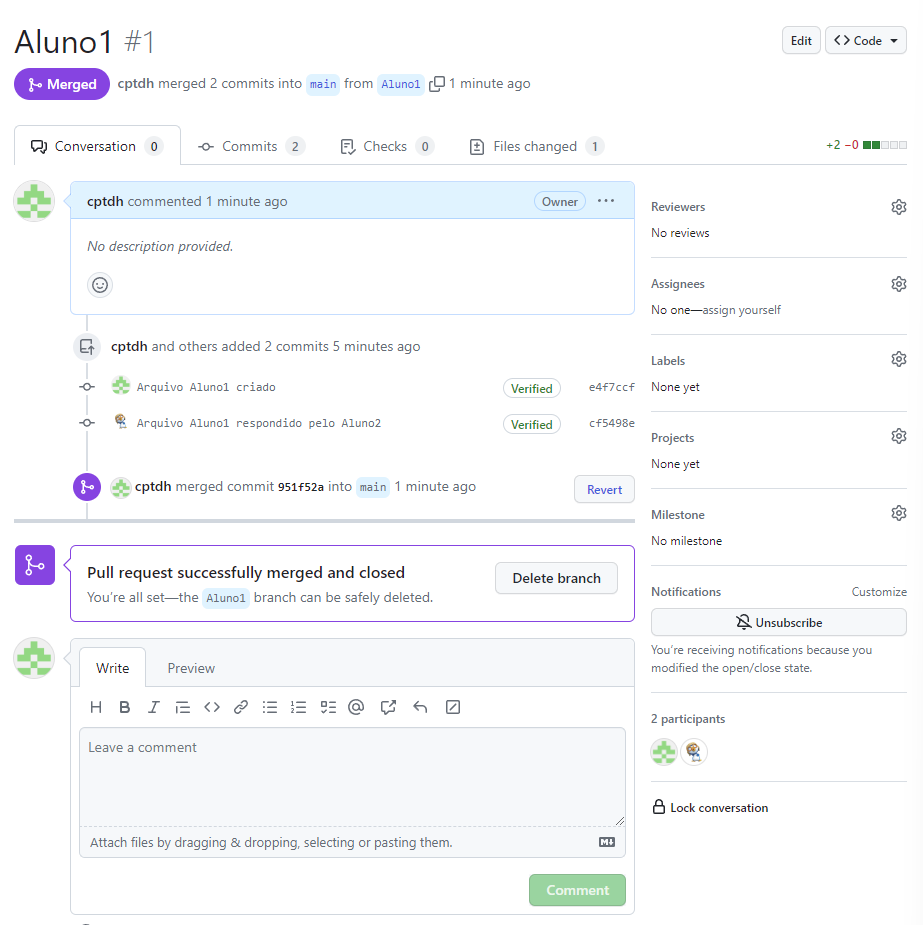
\includegraphics[width=0.5\textwidth]{assets/aula-tdsi-ifds-2023-06-20/Captura de tela 2023-06-19 024507.png}}
            \caption{Merge github}
        \end{figure}
\end{frame}

\begin{frame}[fragile]{Merge do Aluno2}
      \begin{figure}[H]
            \centerline{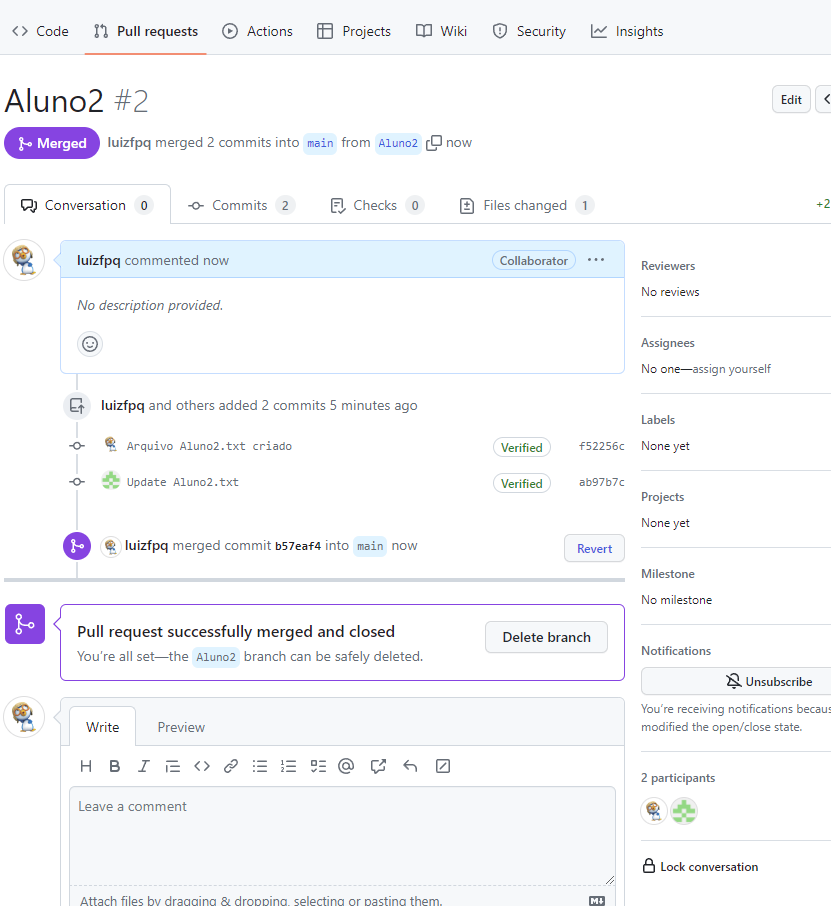
\includegraphics[width=0.5\textwidth]{assets/aula-tdsi-ifds-2023-06-20/Captura de tela 2023-06-19 024520.png}}
            \caption{Merge github}
        \end{figure}
\end{frame}

\begin{frame}[fragile]{Tela principal do repositório}
      \begin{figure}[H]
            \centerline{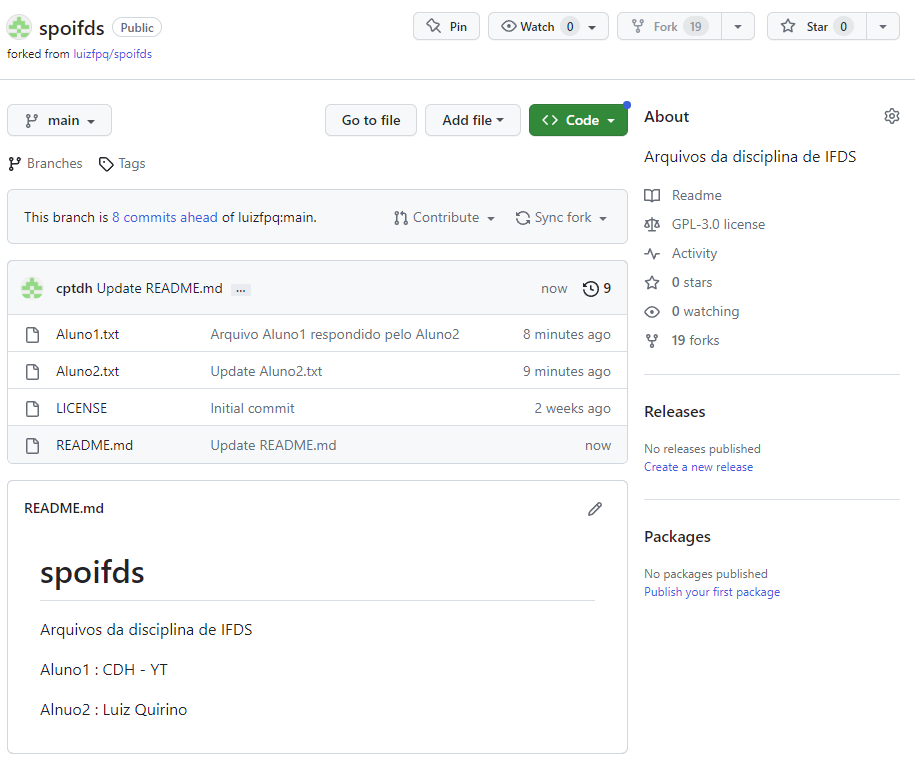
\includegraphics[width=0.5\textwidth]{assets/aula-tdsi-ifds-2023-06-20/Captura de tela 2023-06-19 025033.png}}
            \caption{Tela principal do repositório}
        \end{figure}
\end{frame}

\begin{frame}[fragile]{Tela de histórico de commits}
      \begin{figure}[H]
            \centerline{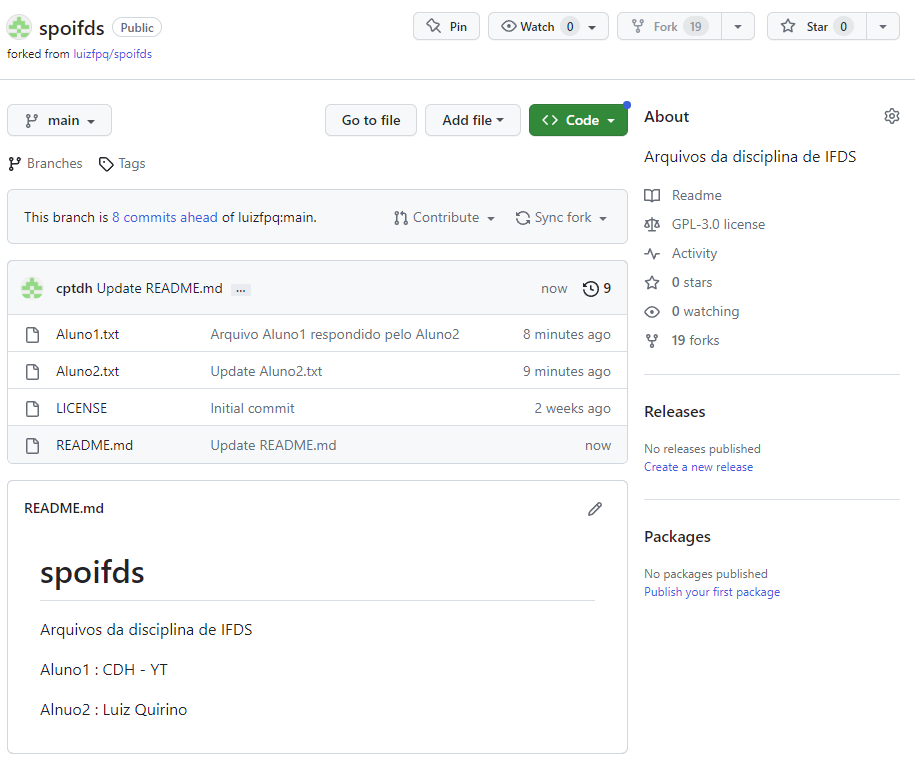
\includegraphics[width=0.5\textwidth]{assets/aula-tdsi-ifds-2023-06-20/Captura de tela 2023-06-19 025033.png}}
            \caption{Tela principal do repositório}
        \end{figure}
\end{frame}

\section{Ajudas e Tira dúvidas}

\begin{frame}{Vídeos de referência}
      \begin{itemize}
            \item \hrefcol{https://youtu.be/di1Fs2GKcD0}{Vídeo ajuda etapa 1: https://youtu.be/di1Fs2GKcD0}
            \item \hrefcol{https://youtu.be/01AsxsLrrp4}{Vídeo ajuda etapa 2: https://youtu.be/01AsxsLrrp4}
            \item \hrefcol{https://youtu.be/Ui-C-A7QL-k}{Vídeo ajuda etapa 3 Parte 1: https://youtu.be/Ui-C-A7QL-k}
            \item \hrefcol{https://youtu.be/Eyu7qS4T_go}{Vídeo ajuda etapa 3 Parte 2: https://youtu.be/Eyu7qS4T\_go}
      \end{itemize}
\end{frame}
\section{Competências desejadas}
\begin{frame}[fragile]{O que será avaliado}
      \begin{itemize}
            \item Sua absorção do conteúdo até o momento para nivelamento;
            \item Seu comprometimento com os compromissos assumidos;
            \\ \textcolor{sintefdarkgreen}{ \textit{* Lembre-se, quanto maior a equipe, maiores responsabilidades, como combinamos}}
            \item Sua atenção aos detalhes apresentados;
            \item Acertividade na execução da tarefa.
      \end{itemize}
\end{frame}



\backmatter
\end{document}
